\hyphenation{аудио-драмах}
\hyphenation{аудио-записях}

\chapter{Аниме: загадочный и поразительный мир японской анимации}
Статья посвящена исследованию объекта Викиданных «аниме». С помощью SPARQL-запросов, вычисляемых на объектах типа «аниме»
в Викиданных, решены такие задачи: выведен упорядоченный список сэйю по числу озвученных ими аниме, построена гистограмма по числу сэйю, озвучивших одно и более аниме, построен граф, связывающий сэйю и озвученные ими аниме, исследован возраст, в котором сэйю озвучивают аниме. 

\marginnote[0.0cm]{Сэйю — это японские актёры озвучивания. Сэйю обычно озвучивают роли персонажей в аниме, видеоиграх, фильмах, а также на радио и телевидении, или выступают в роли рассказчика в радиопостановках и аудиодрамах. Кроме того, голоса сэйю используются в рекламе, голосовых объявлениях, аудиозаписях книг и учебных материалов, а также для переозвучивания. Сэйю могут быть как мужчины, так и женщины.}

\begin{marginfigure}[0.0cm]
{
	\setlength{\fboxsep}{0pt}%
	\setlength{\fboxrule}{1pt}%
	\fcolorbox{gray}{gray}{
\includegraphics{chapter/anime/seyu.jpg}}
}
\caption
[Сэйю]
{
Сэйю Кэндзи Акабанэ озвучивал роль персонажа Sasuke Sarutobi в видеоигре Ikemen Sengoku.\newline
2018 / numan / CC BY-SA 3.0
}
\label{fig:seyu}
\end{marginfigure}

\label{ch:anime}

\section{Экземпляры объекта «Аниме»}

Аниме — это японская анимация. У каждого аниме есть свои актёры озвучивания. В дальнейшем под «сэйю» будем понимать японского актёра озвучивания. В японской анимации слова «актёры озвучивания» и «сэйю» являются синонимами \cite{seiyu_def}. Под словом «тайтл» (от англ. «title», название) обычно понимают конкретное аниме \cite{anime_social}. В общем же смысле слово «тайтл» означает понятие, объединяющее различные виды продукции (от кинофильма до романа), созданные на основе конкретного произведения, за которым закреплено строго определённое название \cite{anime_title_def}.

\begin{itemize}
	\item Свойство: экземпляр (\href{https://www.wikidata.org/wiki/Property:P31}{P31})
	\item Объект: аниме (\href{https://www.wikidata.org/wiki/Q1107}{Q1107})
\end{itemize}

Если получить только список аниме, без учёта подклассов, с помощью такого запроса:

\begin{lstlisting}[ language=SPARQL, 
                    caption={\href{https://w.wiki/4ABw}{Список аниме без учёта подклассов.}\protect\footnotemark},
                    label=lst:anime,
                    texcl 
                    ]
# List of instances of anime
SELECT ?anime ?animeLabel
WHERE
{
    ?anime wdt:P31 wd:Q1107. # instance of anime
    SERVICE wikibase:label{bd:serviceParam
					     wikibase:language "ru,en,ja"}
}
\end{lstlisting}%
\footnotetext{Получено \num{216} результатов в 2021 году. Ссылка на SPARQL-запрос: \href{https://w.wiki/4ABw}{https://w.wiki/4ABw}}

В действительности в Викиданных объектов аниме гораздо больше, но они являются экземплярами не объекта «аниме», а его подклассов. Чтобы получить список жанров аниме и количество аниме, относящихся к этим жанрам, можно выполнить такой запрос:

\begin{lstlisting}[ language=SPARQL, 
                    caption={\href{https://w.wiki/4ABj}{Список жанров аниме и количество аниме, относящихся к этим жанрам.}\protect\footnotemark},
                    label=lst:anime_w_subclass,
                    texcl 
                    ]
# Select anime and its subclasses with number of titles
# corresponding to these subclasses
SELECT ?subAnime ?subAnimeLabel (COUNT(?subAnimeInst) AS ?count)
WHERE {
  ?subAnime wdt:P279* wd:Q1107.       # select anime subclass list
  ?subAnimeInst wdt:P31 ?subAnime # link titles and subclasses
    SERVICE wikibase:label{bd:serviceParam
					     wikibase:language "ru,en,ja"}
}
GROUP BY ?subAnime ?subAnimeLabel
ORDER BY DESC(?count)
\end{lstlisting}%
\footnotetext{Получено \num{11} результатов в 2021 году. Ссылка на SPARQL-запрос: \href{https://w.wiki/4ABj}{https://w.wiki/4ABj}}

Эта классификация не идеальна, так как есть большое смещение в сторону аниме-сериалов: из 4757 тайтлов 2917 отнесены к жанру «аниме-сериал» (61,3 \%); вероятно, классификация жанров аниме в Викиданных требует дальнейшего уточнения. Также в подклассы попали понятия, относящиеся не к общей классификации, а к отдельным аниме, например, \href{https://clck.ru/9cFfS}{«Евангелион»}.

Получим список всех аниме, включая тайтлы, относящиеся к жанрам аниме:

\begin{lstlisting}[ language=SPARQL, 
                    caption={\href{https://w.wiki/49zY}{Список всех аниме на Викиданных.}\protect\footnotemark},
                    label=lst:all_anime_list,
                    texcl 
                    ]
# List of instances of anime and subclasses of anime
SELECT ?anime ?animeLabel
WHERE
{
    ?anime wdt:P31/wdt:P279* wd:Q1107. # instance of anime/subclass
    SERVICE wikibase:label{bd:serviceParam
					     wikibase:language "ru,en,ja"}
}
\end{lstlisting}%
\footnotetext{Получено \num{683} результата в 2017 году и \num{4757} результатов в 2021 году. Ссылка на SPARQL-запрос: \href{https://w.wiki/49zY}{https://w.wiki/49zY}}

Аниме, о которых есть наиболее полная информация на Викиданных: \href{https://www.wikidata.org/wiki/Q4277}{Гуррен-Лаганн}, \href{https://www.wikidata.org/wiki/Q4292}{Space Battleship Yamato}, \href{https://www.wikidata.org/wiki/Q4316}{Project A-ko}

Аниме с малоинформативными записями на Викиданных: \href{https://www.wikidata.org/wiki/Q18692527}{Charlotte}, \href{https://www.wikidata.org/wiki/Q20043638}{Dagashi Kashi}, \href{https://www.wikidata.org/wiki/Q19750843}{KonoSuba}

Среди всех аниме-тайтлов в Викиданных больше всего свойств по данным сервиса ProWD у \href{https://www.wikidata.org/wiki/Q1004318}{Fullmetal Alchemist: The Sacred Star of Milos} (23 свойства).

\subsection{Упорядоченный список сэйю по числу озвученных ими аниме}

Практически в любом аниме присутствуют несколько сэйю. Большинство сэйю озвучили за свою карьеру несколько тайтлов, а многие даже несколько десятков тайтлов. Талантливых сэйю приглашают озвучивать сразу несколько персонажей в одном аниме. Одним из самых популярных сэйю является \href{https://clck.ru/YSCoP}{Хироси Камия}, который за свою карьеру принял участие в озвучке более 180 аниме. Самым известным аниме с его участием является \href{https://clck.ru/YSCrG}{«Атака титанов»}, где он озвучил одного из главных персонажей — капитана Леви.

Построим упорядоченный список сэйю по числу озвученных ими аниме. 

\begin{lstlisting}[ language=SPARQL, 
                    caption={\href{https://w.wiki/49zz}{Упорядоченный список сэйю по числу озвученных ими аниме.}\protect\footnotemark},
                    label=lst:seiyu_titles_sorted,
                    texcl 
                    ]
# Ordered list of seiyu according to the number of anime
# where they took part in
SELECT ?seiyu (SAMPLE(?label) AS ?seiyuLabel) (COUNT(?anime) AS ?count)
WHERE
{
  ?anime wdt:P31/wdt:P279* wd:Q1107;	 # instance of anime/subclass
         wdt:P725 ?seiyu. 	             # instance of seiyu
  ?seiyu rdfs:label ?label	             # subclass of label
    SERVICE wikibase:label{bd:serviceParam
					     wikibase:language "ru,en,ja"}
}
GROUP BY ?seiyu		    # group by seiyu 
ORDER BY DESC(?count)	# order by count of voiced anime
\end{lstlisting}%
\footnotetext{Получено \num{148} результатов в 2017 году и \num{2684} результата в 2021 году. Ссылка на SPARQL-запрос: \href{https://w.wiki/49zz}{https://w.wiki/49zz}}

\subsection{Гистограмма по числу сэйю, озвучивших одно и более аниме}

Было бы интересно построить гистограмму (линейную диаграмму) из сэйю, озвучивших аниме (чем больше аниме озвучил сэйю, тем дальше на диаграмме он будет находиться, «правее» в данном случае).

\begin{lstlisting}[ language=SPARQL, 
                    caption={\href{https://w.wiki/4HFv}{Построение гистограммы по числу сэйю, озвучивших одно и более аниме}\protect\footnotemark},
                    label=lst:seiyu_titles_hist,
                    texcl 
                    ]
# Histogram of the number of seiyu who acted in one or more anime
#defaultView:LineChart
SELECT ?haveseiyu (COUNT(?haveseiyu) AS ?quantity) WHERE {
  {
     SELECT (COUNT(?seiyu) AS ?haveseiyu) WHERE {
       ?anime wdt:P31/wdt:P279* wd:Q1107;
              wdt:P725 ?seiyu.
    SERVICE wikibase:label{bd:serviceParam
					     wikibase:language "ru,en,ja"}
     }
     GROUP BY ?anime             # group list by number of voiced anime
     ORDER BY DESC(?haveseiyu) 
  }
}
GROUP BY ?haveseiyu              # group anime by seiyu quantity
ORDER BY DESC(?haveseiyu)        # order by seiyu quantity (descending)
\end{lstlisting}%
\footnotetext{Получено \num{13} результатов в 2017 году и \num{58} результатов в 2021 году. Ссылка на SPARQL-запрос: \href{https://w.wiki/4HFv}{https://w.wiki/4HFv}}

Очевидно, что чем большее количество аниме берётся в расчёт, тем меньшее количество сэйю участвует в озвучке (рис. ~\ref{fig:Seiyu_histogram_2021_ru}). Многие сэйю, как показано на диаграмме, озвучили только одно аниме. Это может быть связано с неполнотой Викиданных.

\begin{figure*}[h]

    \setlength{\fboxsep}{0pt}%
    \setlength{\fboxrule}{1pt}%
    \fcolorbox{gray}{gray}{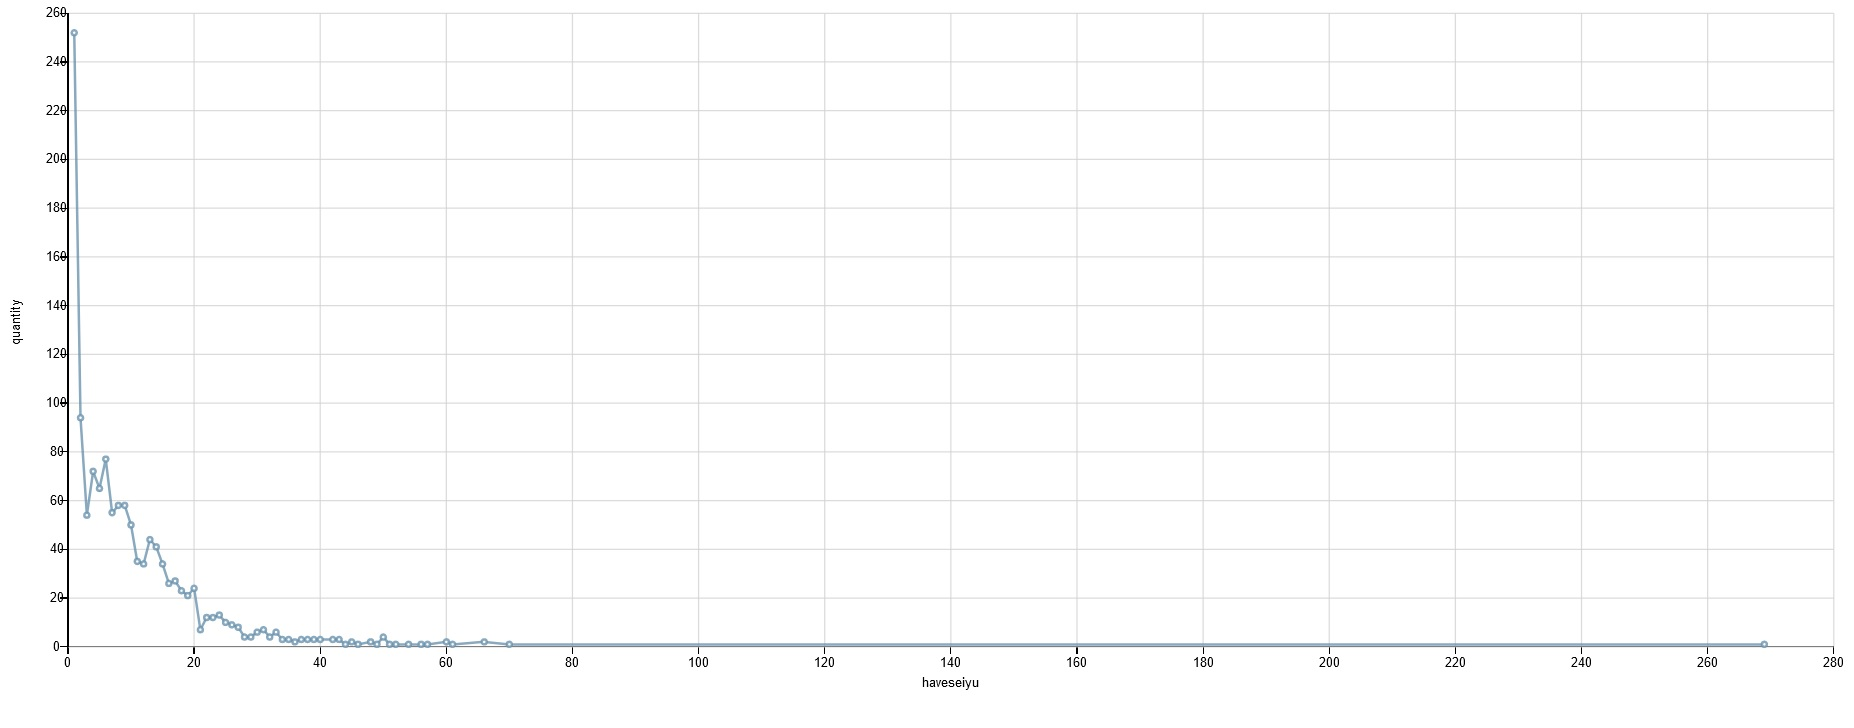
\includegraphics[width=\linewidth]{./chapter/anime/Seiyu_histogram_2021_ru.jpg}}
	\caption[Гистограмма, которая показывает число аниме, озвученных различными сэйю, 2021.]{Гистограмма, которая показывает число аниме, озвученных различными сэйю, 2021. Гистограмма построена на основе данных, полученных с помощью запроса~\protect\ref{lst:seiyu_titles_hist}.}%
    \label{fig:Seiyu_histogram_2021_ru}%
\end{figure*} 

\subsection{Граф, связывающий сэйю и озвученные ими аниме}

Как было сказано ранее, некоторые сэйю могут озвучивать сразу нескольких персонажей в одном аниме или озвучивать несколько аниме. Построим граф, связывающий сэйю и озвученные ими аниме, чтобы нагляднее показать эту взаимосвязь (рис. ~\ref{fig:Seiyu_graph_2021_ru}). 

\begin{lstlisting}[ language=SPARQL, 
                    caption={\href{https://w.wiki/4HFt}{Построение графа, связывающего сэйю и озвученные ими аниме}\protect\footnotemark},
                    label=lst:seiyu_graph,
                    texcl 
                    ]
# Graph of seiyu with more than one anime
#defaultView:Graph
SELECT DISTINCT ?item ?itemLabel ?rgb ?link
WHERE
{ # voice actors (seiyu) with more than one anime
  VALUES ?toggle { true false }
  VALUES ?seiyu { wd:Q6381410 wd:Q1347031 wd:Q1207010 
           wd:Q233902  wd:Q1323728 wd:Q2440809 
           wd:Q355173  wd:Q957795  wd:Q50033}
  ?anime  wdt:P31/wdt:P279* wd:Q1107; # instance of anime/subclass
          wdt:P725 ?seiyu;            # seiyu who voiced this anime 
    SERVICE wikibase:label{bd:serviceParam
					     wikibase:language "ru,en,ja"}
  BIND(IF(?toggle,?anime,?seiyu) AS ?item).
  BIND(IF(?toggle,?animeLabel,?seiyuLabel) AS ?itemLabel).
  BIND(IF(?toggle,"FFFFFF","7FFF00") AS ?rgb).
  BIND(IF(?toggle,"",?anime) AS ?link).
}
\end{lstlisting}%
\footnotetext{Получено \num{826} результатов в 2017 году и \num{494} результата в 2021 году. Ссылка на SPARQL-запрос: \href{https://w.wiki/4HFt}{https://w.wiki/4HFt}}

\begin{figure*}[h]
	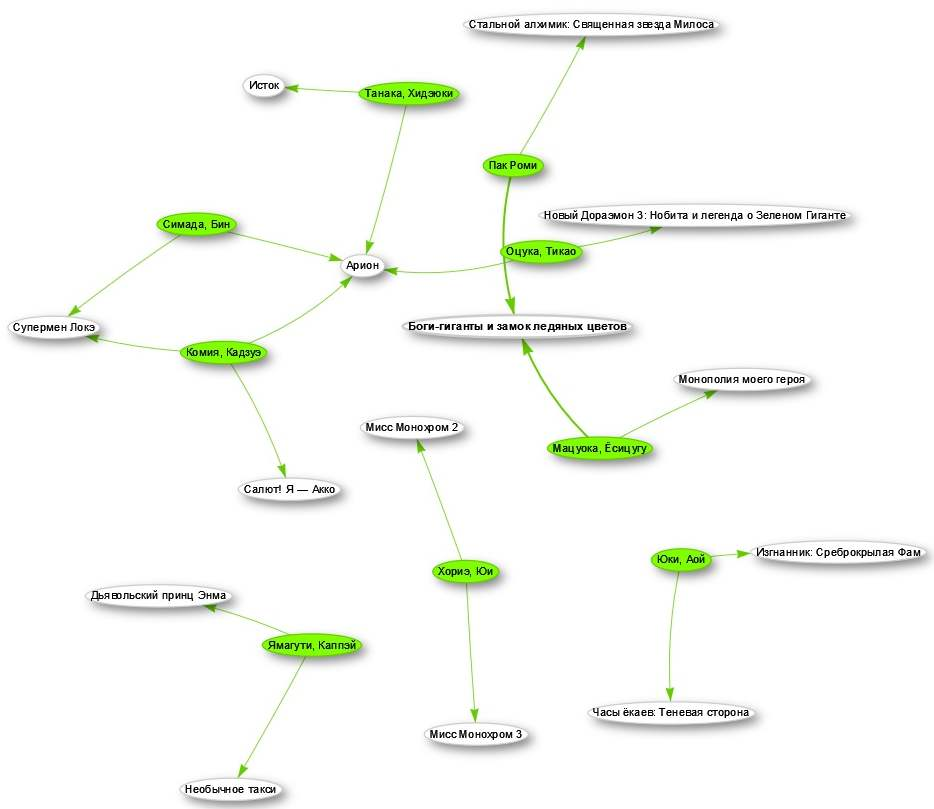
\includegraphics[width=0.72\textwidth]{./chapter/anime/Seiyu_graph_2021_ru.jpg}
	\caption[Фрагмент графа, связывающего сэйю и озвученные ими аниме, 2021.]{Фрагмент графа, связывающего сэйю и озвученные ими аниме, 2021. Граф построен на основе данных, полученных с помощью запроса~\protect\ref{lst:seiyu_graph}.}%
      \label{fig:Seiyu_graph_2021_ru}%
\end{figure*} 

\section{Полнота Викиданных}

\href{https://clck.ru/YTPf9}{Русская Википедия} содержит список тайтлов, состоящий из порядка \num{1638} аниме. Также можно посмотреть \href{https://clck.ru/YTPgk}{телевизионные показы аниме в России по годам}.

В \href{https://en.wikipedia.org/wiki/Lists_of_anime}{Английской Википедии} можно наблюдать примерно такой же результат. Можно просмотреть все аниме с помощью \href{https://en.wikipedia.org/wiki/Category:Lists_of_anime_by_genre}{категорий аниме}, которых на данный момент \num{17}.

На сайте \href{https://shikimori.one/}{Shikimori} в списке аниме \num{801} страница по \num{20} наименований. Нетрудно посчитать, что на сайте есть информация о \num{16020} тайтлах, в то время как в Викиданных объектов, описывающих аниме, всего \num{4756}. К тому же, стоит учитывать, что скорость выхода новых аниме довольно велика. Из этого можно сделать вывод, что Викиданные крайне неполно отражают данные. То же самое касается и жанров: в \href{https://shikimori.one/animes}{разделе поиска Shikimori} доступны \num{42} жанра аниме, в то время как Викиданные содержат информацию только о \num{17}.

Возможно, приведённые ниже статьи и сайты не будут являться \href{https://clck.ru/FLzh8}{АИ}, но с их помощью можно проанализировать информацию об имеющихся аниме и сделать дополнительные выводы о неполноте Викиданных.

\begin{itemize}
	\item На сайте \href{http://online.anidub.best/}{AniDub} приведён список из \num{5756} аниме.
	\item На сайте \href{http://animespirit.tv/}{AnimeSpirit} приведён список из \num{1968} аниме.
	\item На сайте \href{http://animeland.su/}{AnimeLand} приведён список из \num{4795} аниме.
	\item На сайте \href{https://anistar.ew.r.appspot.com/}{AniStar} приведён список из \num{4360} аниме.
	\item На сайте \href{https://anivost.org/}{Anivost} приведён список из \num{420} аниме.
\end{itemize}

Можно сделать вывод, что различные сайты имеют разную информацию об имеющихся аниме. Какие-то сайты появились позже, какие-то раньше, поэтому количество аниме на них может разниться, причём довольно серьёзно. Если упорядочить все приведённые сайты, данные Русской Википедии, Английской Википедии и Викиданные по количеству аниме, то Викиданные окажутся не на последнем месте, но, например, сайту \href{https://shikimori.one/}{Shikimori} они уступают почти в 4 раза. На Викиданных нельзя найти все популярные и известные японские анимации мира, что ещё раз говорит о неполноте.

Вспомним ранее упомянутый запрос, в котором говорилось о \num{2684} сэйю на Викиданных. Дело в том, что поиск производился только по актёрам озвучивания, связанным с аниме, поэтому результат оказался таким скромным. Если запросить информацию о всех актёрах озвучивания (то есть убрать ограничение на категорию аниме), то результат может измениться. 

\begin{lstlisting}[ language=SPARQL, 
                    caption={\href{https://w.wiki/49v2}{Получение списка актёров озвучки и числа озвученных ими проектов}\protect\footnotemark},
                    label=lst:voice_actors_list,
                    texcl 
                    ]
# Ordered list of actors according to the quantity of projects
# voiced by them
SELECT ?actor (SAMPLE(?label) AS ?actorLabel) (COUNT(?anime) AS ?count)
WHERE
{
  ?anime wdt:P725 ?actor.	 # instance of voice actor
  ?actor rdfs:label ?label	 # subclass of label
  FILTER(LANG(?label) = "ru")
}
GROUP BY ?actor		    # group by actor
ORDER BY DESC(?count)	# order by number of voiced anime
\end{lstlisting}%
\footnotetext{Получено \num{3965} результатов в 2017 году и \num{9607} результата в 2021 году. Ссылка на SPARQL-запрос: \href{https://w.wiki/49v2}{https://w.wiki/49v2}}

Такой результат говорит о том, что сэйю могут озвучивать не только аниме, но и другие проекты, и это нужно учитывать при формировании запросов. 

\section{Указана ли дата публикации у аниме?}

Каждый любитель японской анимации желает знать, в каком году вышло его любимое аниме. Викиданные располагают этой информацией не в полной мере. Напишем скрипт, который бы показывал количество аниме с незаполненным полем "publication date" (дата публикации). 

\begin{lstlisting}[ language=SPARQL, 
                    caption={\href{https://w.wiki/4Hcz}{Получение списка аниме, у которых не указана дата выхода на Викиданных}\protect\footnotemark},
                    label=lst:anime_no_pub_date,
                    texcl 
                    ]
# List of anime the release date of which is empty
SELECT ?anime ?animeLabel
WHERE
{
    ?anime wdt:P31/wdt:P279* wd:Q1107;                # instance of anime
    FILTER NOT EXISTS { ?anime wdt:P577 [] }
    SERVICE wikibase:label{bd:serviceParam
					     wikibase:language "ru,en,ja"}
}
\end{lstlisting}%
\footnotetext{Получено \num{237} результатов в 2017 году и \num{2940} результатов в 2021 году. Ссылка на SPARQL-запрос: \href{https://w.wiki/4Hcz}{https://w.wiki/4Hcz}}

\section{Анализ возраста, в котором сэйю озвучивают аниме}

Как и в любой другой профессии, у актёра озвучки есть возраст, когда он находится в «расцвете сил» и может озвучить множество аниме, а через несколько лет — «подать в отставку». Использование SPARQL и внешних инструментов для анализа данных, таких как \href{https://ru.wikipedia.org/wiki/Python}{язык программирования Python}, может позволить оценить такой возраст на основе информации из Викиданных.

Чтобы получить исходные данные для исследования, необходимо выполнить три SPARQL-скрипта и экспортировать результаты их выполнения в формате \href{https://ru.wikipedia.org/wiki/CSV}{.csv}.

Получить список всех зарегистрированных в Викиданных сэйю и их дат рождения можно двумя способами: 

\begin{lstlisting}[ language=SPARQL, 
                    caption={\href{https://w.wiki/4FPq}{Получение дат рождения сэйю (вариант 1)}\protect\footnotemark},
                    label=lst:seiyu_bd_w_service,
                    texcl 
                    ]
# Get list of all seiyu objects, their names and birth dates
SELECT ?seiyu ?seiyuLabel ?bDate WHERE {
  ?anime (wdt:P31/(wdt:P279*)) wd:Q1107;
    wdt:P725 ?seiyu.       # seiyu is anime voice actors
  ?seiyu wdt:P569 ?bDate.  #       has a birthday
    SERVICE wikibase:label{bd:serviceParam
					     wikibase:language "ru,en,ja"}
}
GROUP BY ?seiyu ?seiyuLabel ?bDate
\end{lstlisting}%
\footnotetext{Получено \num{2515} результатов в 2021 году. Ссылка на SPARQL-запрос: \href{https://w.wiki/4FPq}{https://w.wiki/4FPq}}

\begin{lstlisting}[ language=SPARQL, 
                    caption={\href{https://w.wiki/4FPn}{Получение дат рождения сэйю (вариант 2)}\protect\footnotemark},
                    label=lst:seiyu_bd_w_rdfs,
                    texcl 
                    ]
# Get list of all seiyu objects, their names and birth dates
SELECT ?seiyu (SAMPLE(?seiyu) AS ?seiyuLabel) ?bDate WHERE {
  ?anime (wdt:P31/(wdt:P279*)) wd:Q1107;
    wdt:P725 ?seiyu.       # seiyu is anime voice actors
  ?seiyu wdt:P569 ?bDate.  #       has a birthday 
  ?seiyu rdfs:label ?label.
}
GROUP BY ?seiyu ?bDate
\end{lstlisting}%
\footnotetext{Получено \num{2515} результатов в 2021 году. Ссылка на SPARQL-запрос: \href{https://w.wiki/4FPn}{https://w.wiki/4FPn}}

Различия между скриптами:

\begin{itemize}
    \item метка (имя) сэйю в первом случае получается с помощью переменной ?seiyuLabel (в таком случае нужно указать команду SERVICE для установки языков, на котором будут возвращены имена), а во втором - с помощью конструкции rdfs:label;
    \item в первом варианте скрипта необходимо указывать ?seiyuLabel как параметр GROUP BY, чтобы связать объекты сэйю и их метки.
\end{itemize}

Получение списка всех зарегистрированных в Викиданных аниме и дат их выхода: 

\begin{lstlisting}[ language=SPARQL, 
                    caption={\href{https://w.wiki/4ENc}{Получение дат выхода аниме}\protect\footnotemark},
                    label=lst:all_anime_releases,
                    texcl 
                    ]
# Get all anime objects, their names and release dates
SELECT ?anime ?animeLabel ?animePubDate ?animeSeriesStartDate
WHERE {
  ?anime (wdt:P31/(wdt:P279*)) wd:Q1107.               # object of anime/subclass
  OPTIONAL { ?anime wdt:P577 ?animePubDate. }          # release date of a movie
  OPTIONAL { ?anime wdt:P580
					?animeSeriesStartDate. }  # start date of a series
    SERVICE wikibase:label{bd:serviceParam
					     		wikibase:language "ru,en,ja"}
}
\end{lstlisting}%
\footnotetext{Получено \num{5264} результатов в 2021 году. Ссылка на SPARQL-запрос: \href{https://w.wiki/4ENc}{https://w.wiki/4ENc}}

Обратите внимание, что скрипт получает не только даты выхода полнометражных аниме (свойство P577), но и даты начала показа сериалов (свойство P580). 

Получение ссылок между объектами сэйю и аниме, которые они озвучивали: 

\begin{lstlisting}[ language=SPARQL, 
                    caption={\href{https://w.wiki/4ELh}{Получение ссылок между сэйю и аниме}\protect\footnotemark},
                    label=lst:link_anime_seiyu,
                    texcl 
                    ]
# List of links between seiyu and anime where they are involved in
SELECT DISTINCT ?item ?itemLabel ?link ?itemType
WHERE
{
  VALUES ?toggle { true false }
  ?anime  wdt:P31/wdt:P279* wd:Q1107; # instance of anime/subclass
          wdt:P725 ?seiyu.            # list seiyu who acted in this anime
  
  BIND(IF(?toggle,?anime,?seiyu) AS ?item).   # anime/seiyu link
  BIND(IF(?toggle,?animeLabel,?seiyuLabel)
					AS ?itemLabel).  # anime/seiyu labels link
  BIND(IF(?toggle,?seiyu,?anime) AS ?link).   # seiyu/anime link
  BIND(IF(?toggle,?seiyu,"seiyu")
							AS ?itemType).
    SERVICE wikibase:label{bd:serviceParam
					     		wikibase:language "ru,en,ja"}
}
\end{lstlisting}%
\footnotetext{Получено \num{27092} результата в 2021 году. Ссылка на SPARQL-запрос: \href{https://w.wiki/4ELh}{https://w.wiki/4ELh}}

Результат анализа удобно представить в виде гистограммы. Для её построения можно воспользоваться средствами таких библиотек для Python, как \href{https://ru.wikipedia.org/wiki/Pandas}{Pandas} для обработки табличных данных и \href{https://ru.wikipedia.org/wiki/Matplotlib}{Matplotlib} для непосредственно построения графиков. Код скрипта, создающего гистограмму, опубликован на сервисе \href{https://github.com/componavt/wd_book/blob/master/programming_tasks/seiyu_age/age_act_hist.ipynb}{GitHub}.

В результате получим гистограмму, по оси абсцисс которой отмечен возраст в годах, а по оси ординат — суммарное количество ролей, озвученных всеми сэйю такого возраста. Получившаяся гистограмма представлена на рис. ~\ref{fig:Seiyu_age_hist_RU}. 

\begin{figure*}[h]

    \setlength{\fboxsep}{0pt}%
    \setlength{\fboxrule}{1pt}%
    \fcolorbox{gray}{gray}{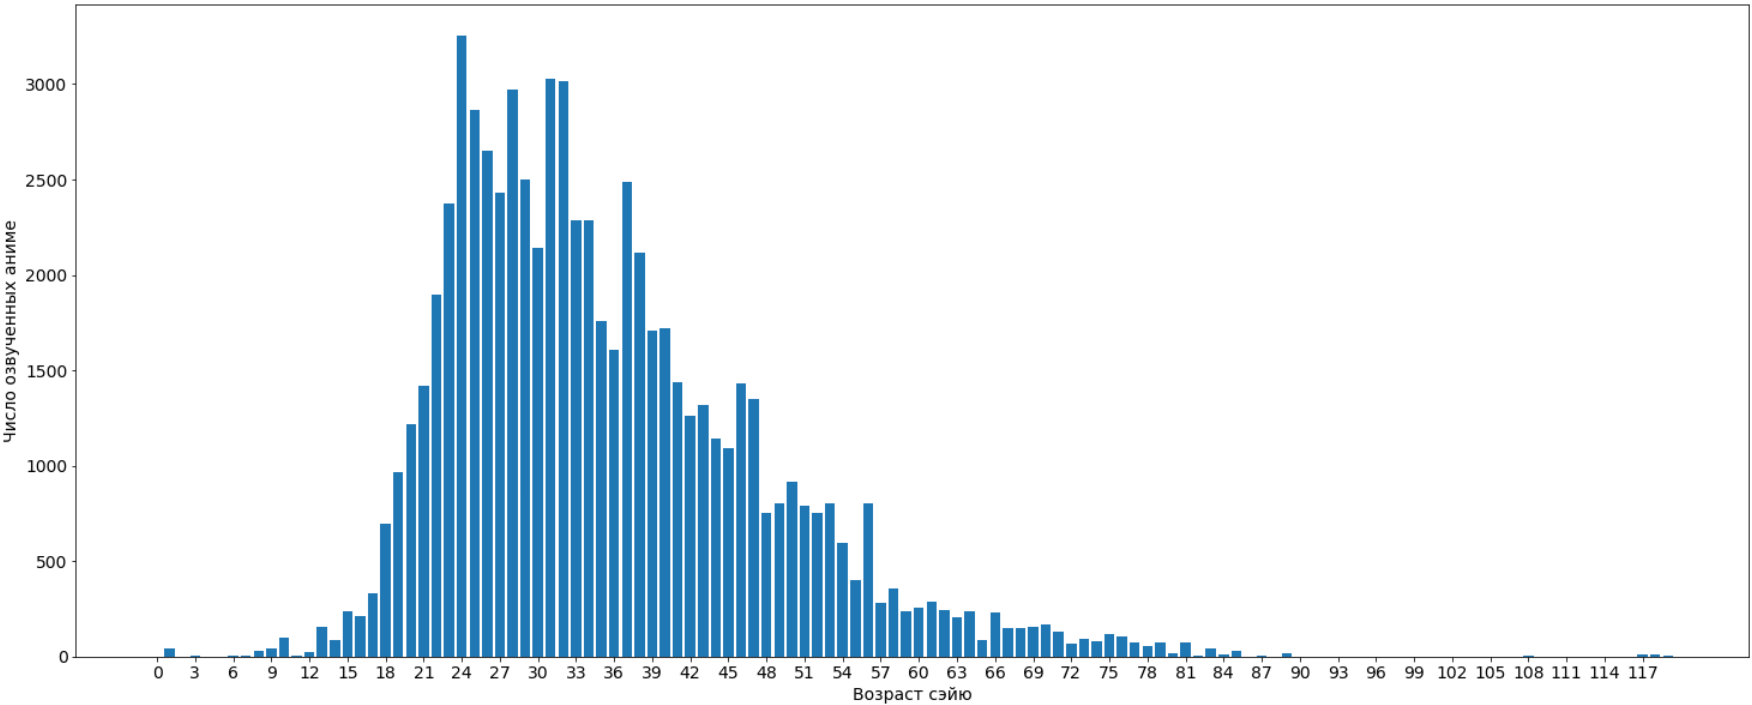
\includegraphics[width=\linewidth]{./chapter/anime/Seiyu_age_hist_RU.png}}
	\caption[Гистограмма, которая отображает число аниме, озвученное сэйю разных возрастов, 2021.]{Гистограмма, которая показывает число аниме, озвученных различными сэйю, 2021. Гистограмма построена на основе данных, полученных с помощью запроса ~\protect\ref{lst:link_anime_seiyu}.}%
    \label{fig:Seiyu_age_hist_RU}%
\end{figure*} 

Интересные наблюдения:
\begin{itemize}
    \item В данных есть забавные моменты, когда сэйю родился(-ась) позже, когда вышло аниме с его (её) участием. Вероятно, это связано с отсутствием информации в Викиданных о втором сезоне/перезапуске аниме. Например, на 2021 год такая ситуация наблюдается для аниме \href{https://www.wikidata.org/wiki/Q11304591}{Sazae-san} и сэйю \href{https://www.wikidata.org/wiki/Q5968283}{Нобунага Симадзаки}.
\end{itemize}

\section{Будущая работа}

\begin{enumerate}
    \item Вывести 10 аниме, выпущенных в 2017 году.
    \item Вывести 5 аниме, в которых число сэйю является наибольшим.
    \item Построить пузырьковую диаграмму (BubbleChart) распределения аниме по жанрам (сколько аниме в каждом жанре).
    \item Отметить на карте места рождения сэйю.
    \item Построить гистограмму или пузырьковую диаграмму национальностей сэйю.
    \item Построить гистограмму количества вышедших аниме по годам или количества сэйю по годам рождения.
\end{enumerate}